\section{Receiver EPS}
\label{receiver_EPS}

The EPS system of the receiver is almost the same as that of the emitter.

Table \ref{tab:receiverPowerBudget} on page \pageref{tab:receiverPowerBudget} gives the power budget for the receiver satellites. The required total power generation for the subsystems is 32.12 W. Again a margin of $15\%$ was taken. This implies that the power system requires 4.9 W to operate resulting in a total power usage of 41.838 W. This resulted in a required solar panel area of 0.5 square meters. Again the STK program was used to verify that the assumed cosine loss value was correct. The calculated power generation for 0.5 square meters was 52.5 W, thus again it is shown that the value was correct.

\begin{table}
\centering
\begin{tabular}{lc}
\hline
Subsystem & Power requirement [W]\\
\midrule
Communications & 28\\
Navigation & 1.12\\
ORP & 0.2\\
ADCS & 2.8\\
\midrule
Total & 32.12\\
Safety margin of $15\%$ & 4.818\\
EPS & 4.9\\
\midrule
\midrule
\textbf{Grand Total} & 41.838}\\
\hline
\end{tabular}
\caption{Receiver power budget}
\label{tab:receiverPowerBudget}
\end{table}

Because the power requirement is much less also the amount of batteries necessary was less. For the receiver, only one battery with 2 modules was needed to be able to power the satellite during eclipse.
\\\\
Table \ref{tab:EPS_detailsRec} shows the dimensions, weight and power usage of each part of the emitter satellite's electrical power system. The losses of the solar panels and batteries are considered in their design, therefore their power use is listed as zero in this table. To achieve a good ballistic coefficient, the mass of the receiver satellites needed to be one kilogram larger without increasing the volume or area of the satellites. It was decided to thicken the Germanium substrate layer of the solar panels by 0.38 mm. This made the panels 1045 grams heavier.

\begin{table}[H!]
\centering
\begin{tabular}{cccccc}
\toprule
Part & \multicolumn{3}{c}{Dimensions [mm]} & Weight [g] & Power usage [W]\\ 
\midrule
 & Length & Width & Height & & \\ 
 Driver (2 needed) & 30 & 6 & 60 & 21.4 & 1 \\ 
 SMA Deployment (2 needed) & 120 & 50 & 10 & 120 & 4* \\ 
 Battery & 168 & 102 & 10 & 1000 & 0 \\ 
 Convertor & 95 & 60 & 17 & 80 & 1.5 \\ 
 Shunt regulator  (2 needed) & 2.8 & 2.6 & 1.05 & 0.1 & 0.5 \\ 
 Thermal knife (2 needed) & 60 & 50 & 38 & 280 & 15**  \\
 Wiring & - & - & - & 230 & 0.28 \\ 
 Solar panels (2 needed) & 500 & 500 & 5.866 & 723.5 & 0 \\
 \midrule
 \textbf{TOTAL} & - & - & - & 3600 & 4.875***  \\ 
\bottomrule
 \multicolumn{6}{l}{* for 4 minutes} \\
 \multicolumn{6}{l}{** for 60 seconds} \\
 \multicolumn{6}{l}{*** continuous power usage only} \\
\end{tabular}
\caption{EPS subpart details for receiver satellites}
\label{tab:EPS_detailsRec}
\end{table}


As with the emitter, here the architecture of the power system of the receiver is show in figure \ref{fig:receiver_block}. The power from the solar panels is transferred to the dc-dc convertor. There part of it is sent to charge the batteries and part is sent to power the payload. During eclipse periods, the power is sent from the batteries to the payload via the convertor.

\begin{figure}[H!]
\centering
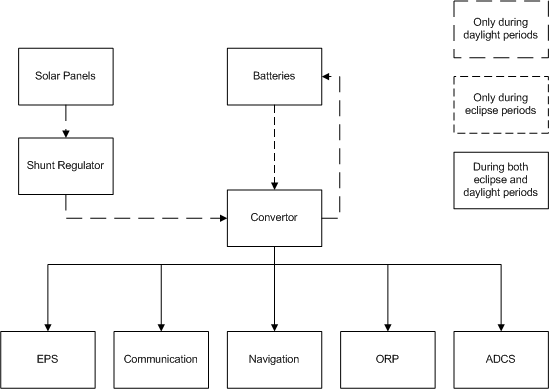
\includegraphics[scale = 0.7]{chapters/img/EPS_receiver_block_diagram.png}
\caption{Electrical block diagram of the receiver}
\label{fig:receiver_block}
\end{figure}